% Straight up stealing preamble from Eli Holmes 
%%%%%%%%%%%%%%%%%%%%%%%%%%%%%%%%%%%%%%START PREAMBLE THAT IS THE SAME FOR ALL EXAMPLES
\documentclass{article}

%Required: You must have these
\usepackage{Sweave}
\usepackage{graphicx}
\usepackage{tabularx}
\usepackage{hyperref}
\usepackage{natbib}
\usepackage{pdflscape}
\usepackage{array}
\usepackage{gensymb}
%\usepackage[backend=bibtex]{biblatex}
%Strongly recommended
  %put your figures in one place
%\SweaveOpts{prefix.string=figures/, eps=FALSE} 
%you'll want these for pretty captioning
\usepackage[small]{caption}

\setkeys{Gin}{width=0.8\textwidth}  %make the figs 50 perc textwidth
\setlength{\captionmargin}{30pt}
\setlength{\abovecaptionskip}{10pt}
\setlength{\belowcaptionskip}{10pt}
% manual for caption  http://www.dd.chalmers.se/latex/Docs/PDF/caption.pdf

%Optional: I like to muck with my margins and spacing in ways that LaTeX frowns on
%Here's how to do that
 \topmargin -1.5cm        
 \oddsidemargin -0.04cm   
 \evensidemargin -0.04cm  % same as oddsidemargin but for left-hand pages
 \textwidth 16.59cm
 \textheight 21.94cm 
 %\pagestyle{empty}       % Uncomment if don't want page numbers
 \parskip 7.2pt           % sets spacing between paragraphs
 %\renewcommand{\baselinestretch}{1.5} 	% Uncomment for 1.5 spacing between lines
\parindent 0pt% sets leading space for paragraphs
\usepackage{setspace}
%\doublespacing

%Optional: I like fancy headers
%\usepackage{fancyhdr}
%\pagestyle{fancy}
%\fancyhead[LO]{How do climate change experiments actually change climate}
%\fancyhead[RO]{2016}
 
%%%%%%%%%%%%%%%%%%%%%%%%%%%%%%%%%%%%%%END PREAMBLE THAT IS THE SAME FOR ALL EXAMPLES

%Start of the document
\begin{document}

%\SweaveOpts{concordance=TRUE}
 \bibliographystyle{/Users/aileneettinger/citations/Bibtex/styles/amnat.bst}
\title{Spatial and temporal shifts in photoperiod with climate change} % perspective paper for OSPREE analyses

\author{A.K. Ettinger, D. Buonaiuto, C. Chamberlain, I. Morales-Castilla, E. Wolkovich}
%\date{\today}%do we need to also add any of the following: D. Flynn, T. Savas, J. Samaha, E. Forrestel? 
\maketitle  %put the fancy title on
%\tableofcontents      %add a table of contents
%\clearpage
%%%%%%%%%%%%%%%%%%%%%%%%%%%%%%%%%%%%%%%%%%%%%%%%%%%
\begin{enumerate}
\item \textit{Introduction}
\begin{enumerate}
\item Photoperiod is a critical cue used by organisms to synchronize their activities with seasonal climatic changes (add other citations- there are many possibilities! if you have favorites, please add along with 1-2 words of what the activity is)\citep[e.g.,][]{hsu2011,singh2017}.
\item As species undergo climate change-induced shifts in space and/or time, the daylength they experience will be altered. 
\item Many experiments have altered photoperiod, often interacting with temperature changes; however, photoperiod treatments in these experiments are not typically designed to be applied to climate change forecasting. 
\item Here, we ask: 
\begin{enumerate}
\item How will climate change alter the photoperiod experienced by organisms, given observed (and forecasted?) biological shifts (both spatial and temporal)?
\item What are the implications of these altered photoperiods for forecasts of climate change impacts?
\item Can the large quantity of experiments altering photoperiod be applied to forecasting biological implications of climate change (i.e. do they occur at the appropriate scale)?
\end{enumerate}
\end{enumerate}

\item\textit{How will climate change alter the photoperiod experienced by organisms?}
\begin{enumerate}
\item Spatial shifts in species ranges and temporal shifts in species phenology and activity will alter the photoperiods experienced by organisms under climate change.
\item  To date, most work has focused on how spatial range shifts with climate change will affect photoperiod \citep{saikkonen2012}, but temporal shifts actually yield bigger changes in experienced photoperiod than spatial shifts  (Figures \ref{fig:photo},\ref{fig:photo_bar}).
\item Shifts in photoperiod may vary with latitude (Figure \ref{fig:photo_bar}). 
\item Photoperiod sensitivity can also vary with latitude (cite OSPREE database and perhaps add a table?), so it is unclear how these two things interact.
\end{enumerate}
\item\textit{What are the implications of these altered photoperiods for forecasts of climate change impacts?}
\begin{enumerate}
\item Phenology will be altered, given that daylength is known to affect vegetative growth, cell elongation, and budburst \citep{linkosalo2006,erwin1998,sidaway2010, hsu2011}.
\item It has been proposed that photoperiod may eventually become a limiting factor, constraining the ability of trees to shift their phenology with warming \citep{koerner2010,vitasse2013, morin2010}. 
\item Interactions between photoperiod and forcing and chilling could result in muted or exaggerated phenological shifts, compared to what would be expected based on temperature change alone. Say something about crossing thresholds of daylength and the "external coincidence model" for photoperiod control \citep{bastow2002,kobayashi2007,andres2012,singh2017}?
\item Effects of photoperiod on forecasting of biological impacts of climate change needs additional investifation. In some forecasting methods (e.g. species distirbution modelling), the role of photoperiod is largely ignored (i think this is true? add some citations). In other cases, photoperiod is incorporated into foreacasts, along with other variables such as evaporative demand, and temperature \citep [e.g. ED] []{jolly2005, medvigy2013}. These models need to be more widely tested, e.g. in different ecosystems/species, and given recent findings about the role of photoperiod in phenology.     
\end{enumerate}
\item\textit{Can existing experiments be applied to forecasting?}
\begin{enumerate}
\item Table of OSPREE experiments that manipulate photoperiod, their daylength treatments, their findings, and perhaps how the treatment corresponds to spatial/temporal shifts?
\item Most experiments manipulate photoperiod much more dramatically than will occur with climate change (but see \citep{basler2012}), so it is difficult to extrapolate findings. (This may not be true for all latitudes- for example high latitudes experience more dramatic changes in photoperiod across the year.)
\item There is a great need to better understand exactly how photoperiod acts as a cue (linear response? threshold? how does it interact with temperature to break dormancy?)
\end{enumerate}
\item\textit{Conclusions}
\begin{enumerate}
\item Organisms may experience large changes to the photoperiod they experience, under climate change, even if they do not shift their ranges.
\item More studies needed with fine-scale changes in photoperiod
\end{enumerate}
\end{enumerate}

\section* {To do:}
\begin{enumerate}
\item Make a map showing daylength or greenup dates globally 
\item Make Table of studies and treatments
\item Make Table of studies testing if photoperiod varies by latitudinal origin
\end{enumerate}
\bibliography{/Users/aileneettinger/citations/Bibtex/mylibrary}
\clearpage
\section* {Tables}
% latex table generated in R 3.4.2 by xtable 1.8-2 package
% Tue Oct 17 11:20:24 2017
\begin{table}[ht]
\centering
\caption{Growth chamber experiments and their photoperiod treatments.} 
\label{table:phototreats}
\begin{tabular}{|p{0.15\textwidth}|p{0.08\textwidth}|p{0.08\textwidth}|p{0.08\textwidth}|p{0.06\textwidth}|p{0.15\textwidth}|}
  \hline
study & lat & long & daylength & space & time \\ 
  \hline
howe95 & 40.548 & -124.097 & 9-24 &  & exceeds range \\ 
  schnabel87 & 46.209 & -119.766 & 9.5-14 &  & -86 \\ 
  nienstaedt66 & 44.166 & -103.916 & 8-20 &  & exceeds range \\ 
  ashby62 & 42.988 & -89.412 & 8-16 &  & exceeds range \\ 
  okie11 & 32.120 & -83.120 & 0-12 &  & exceeds range \\ 
  durner84 & 37.227 & -80.423 & 9-16 &  & exceeds range \\ 
  bradford10 & 42.700 & -75.968 & 9-16 &  & exceeds range \\ 
  worrall67 & 41.306 & -72.928 & 8-16 &  & exceeds range \\ 
  caffarra11a & 52.320 & -6.934 & 8-16 &  & -132 \\ 
  caffarra11b & 52.320 & -6.934 & 10-16 &  & -94 \\ 
  heide05 & 56.176 & -4.316 & 10-24 &  & exceeds range \\ 
  Sanz-Perez09 & 40.400 & -3.480 & 10-16 &  & exceeds range \\ 
  heide12 & 56.500 & -3.062 & 10-24 &  & exceeds range \\ 
  smeets80 & 51.984 & 5.665 & 8-24 &  & exceeds range \\ 
  heide93a & 47.500 & 7.600 & 13-16 &  & -78 \\ 
  basler14 & 46.315 & 8.265 & 9.2-16 &  & Inf \\ 
  myking95 & 56.100 & 9.150 & 8-24 &  & exceeds range \\ 
  heide77 & 56.074 & 9.379 & 10-16 &  & -79 \\ 
  heide11 & 59.667 & 10.667 & 10-20 &  & Inf \\ 
  falusi90 & 46.033 & 10.750 & 9-13 &  & -82 \\ 
  heide93 & 59.500 & 10.767 & 8-24 &  & exceeds range \\ 
  myking97 & 59.667 & 10.767 & 12-24 &  & Inf \\ 
  pettersen71 & 59.660 & 10.770 & 10-24 &  & exceeds range \\ 
  sonsteby06 & 59.666 & 10.792 & 10-24 &  & exceeds range \\ 
  heide93a & 59.670 & 10.830 & 8-24 &  & exceeds range \\ 
  heide01 & 59.666 & 11.333 & 10-24 &  & exceeds range \\ 
  ghelardini10 & 43.717 & 11.367 & 8-16 &  & exceeds range \\ 
  zohner16 & 48.164 & 11.503 & 8-16 &  & exceeds range \\ 
  laube14a & 48.403 & 11.712 & 8-16 &  & exceeds range \\ 
  heide08 & 48.396 & 11.725 & 10-24 &  & exceeds range \\ 
  sogaard08 & 60.278 & 12.734 & 12-24 &  & Inf \\ 
  falusi96 & 38.267 & 15.988 & 9-13 &  & Inf \\ 
  partanen98 & 60.033 & 23.050 & 8.66-12 &  & -37 \\ 
  viheraaarnio06 & 60.450 & 24.930 & 15-19 &  & -62 \\ 
  viheraaarnio06 & 67.730 & 24.930 & 20-23 &  & Inf \\ 
  partanen01 & 61.933 & 26.683 & 6-16 &  & -105 \\ 
  partanen05 & 61.817 & 29.317 & 5-20 &  & exceeds range \\ 
  gutterman88 & 30.850 & 34.770 & 8-24 &  & exceeds range \\ 
  biran73 & 31.890 & 34.819 & 10.5-16 &  & exceeds range \\ 
   \hline
\end{tabular}
\end{table}\clearpage
\begin{table}[p]
  \caption{\textbf{Growth chamber experiments and their photoperiod treatments.} From OSPREE. For now, I used 45.5 lat to estimate spatial and temporal equivalents and Y/N for sensitivity but might be better to have a magnitude of sensitivity found?}
\begin{footnotesize} 
   \begin{tabular}{| p{1cm} | p{3.8cm} | p{2.9 cm} | p{3.2 cm} |}
    \hline
  \bf{Study} & \bf{Photoperiod treatments (or delta)} & \bf{Spatial equivalent} & \bf{Temporal equivalent}\\ \hline
    basler12 & 9.5, 11 (1.5) &  600 km up & 30 days earlier \\ \hline
    laube14a & 8,16 (8) &  3200 km up & 160 days earlier \\ \hline
    other studies &  &   & \\ \hline

     \end{tabular}    
\end{footnotesize} 
    \end{table}
\clearpage
\section* {Figures}
\begin{figure}[p]
\centering
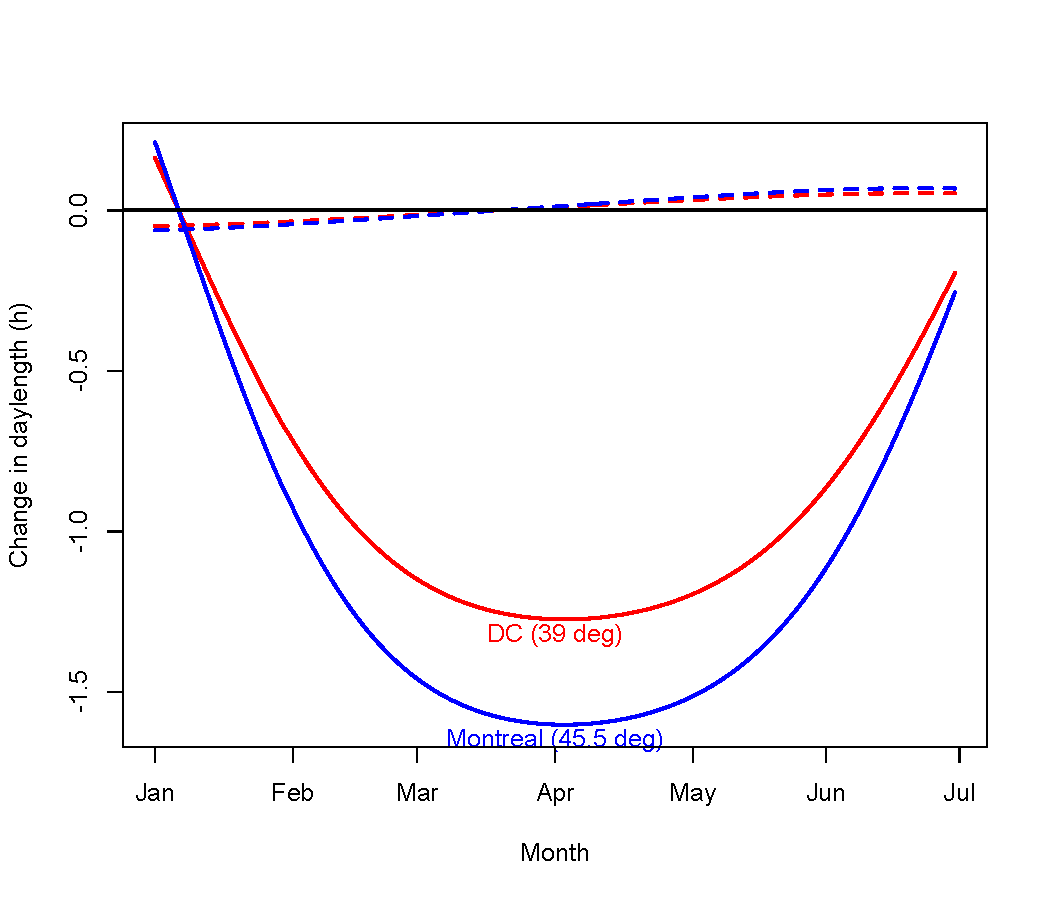
\includegraphics{/Users/aileneettinger/git/ospree/docs/photoperiod/figures/photoper_change.pdf} 
\caption{\textbf{Shifts in the photoperiod organisms will experience with climate change, at two latitudes (Washington, DC and Montreal).}  With warming, species are likely to shift their ranges poleward and/or shift their spring activity earlier, resulting in alterations to the photoperiod they experience. We compare changes to photoperiod in 100 years if species shift spatially (i.e. shifting their ranges ~6km,or 0.05 degree, per decade poleward, solid lines) versus temporally (shifting activity earlier 3 days per decade, dashed lines).}
 \label{fig:photo}
 \end{figure}
\begin{figure}[p]
\centering
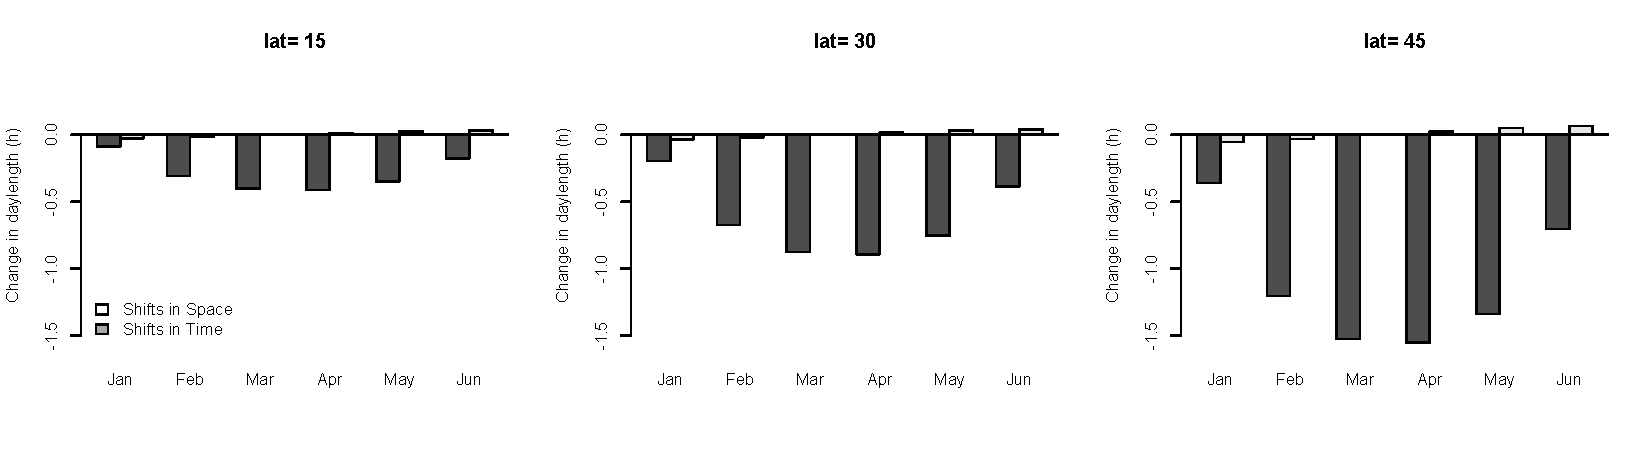
\includegraphics{/Users/aileneettinger/git/ospree/docs/photoperiod/figures/photoper_change_bar.pdf} 
\caption{\textbf{Shifts in the photoperiod organisms will experience with climate change, across latitude.}  With warming, species are likely to shift their ranges poleward and/or shift their spring activity earlier, resulting in alterations to the photoperiod they experience. We compare changes to photoperiod in 100 years if species shift spatially (i.e. shifting their ranges ~6km,or 0.05 degree, per decade poleward) versus temporally (shifting activity earlier 3 days per decade).}
 \label{fig:photo_bar}%Lizzie did not like the bar plot since it is binning a continuous variable. perhaps just include as an inset?
 \end{figure}
\clearpage



%%%%%%%%%%%%%%%%%%%%%%%%%%%%%%%%%%%%%%%%
\end{document}
%%%%%%%%%%%%%%%%%%%%%%%%%%%%%%%%%%%%%%%%
